\documentclass[10pt,a4paper]{article}
\usepackage[utf8]{inputenc}
\usepackage[italian]{babel}
\usepackage{amsmath}
\usepackage{amsfonts}
\usepackage{amssymb}
\usepackage{graphicx}
\usepackage[left=2cm,right=2cm,top=2cm,bottom=2cm]{geometry}
\newcommand{\rem}[1]{[\emph{#1}]}

\author{Gruppo BN \\ Federico Belliardo, Marco Costa, Lisa Bedini}
\title{Ottica 2}
\begin{document}

\maketitle
\section{Scopo dell'esperienza}
L'esperienza si divide in due parti distinte. Nella prima si stima la lunghezza d'onda della radiazione di un laser a diodo mediante la misura degli ordini di diffrazione provocati dall'incidenza sulla scala graduata di un calibro utilizzata come reticolo. Nella seconda parte mediante un laser He-Ne si calibra un interferometro di Michelson per eseguire la misura della lunghezza d'onda della riga verde del mercurio, e in seguito osservare le frange di interferenza con luce bianca.

\section{Materiale occorrente}
\begin{itemize}
\item Calibro
\item Laser a diodo
\item Metro a nastro
\item Interferometro di Michelson
\item Laser He-Ne
\item Lampada al mercurio
\item Filtro verde
\end{itemize}

\section{Parte A - Misura della lunghezza d'onda del laser a diodo}
\subsection{Modalità operative}

\begin{figure}[!htb]
  \centering
  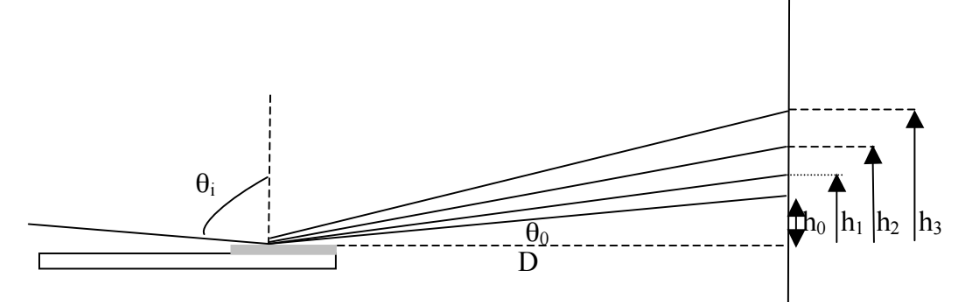
\includegraphics[scale=.5]{disegno1.png}
\caption{Disegno schematico dell'esperimento di diffrazione.}
\label{parteAfigura}

\end{figure}
La spaziatura tra le suddivisioni della scala graduata del calibro è troppo grande per poter essere usata come reticolo di diffrazione per la luce visibile senza l'accorgimento di far incidere il fascio in modo radente alla scala, cioè con angolo di incidenza prossimo a $\frac{\pi}{2}$. Il fascio riflesso e i vari ordini di diffrazione sono visibili un un muro (schermo) a circa due metri di distanza.\\
Sul muro si è posto un foglio di carta su cui si sono segnati il punto in cui il laser sarebbe arrivato se non fosse stato diffratto, il punto in cui il fascio viene riflesso dal calibro e i vari ordini di diffrazione dal calibro. La media delle posizioni del punto di incidenza diretta e del punto di riflessione è la proiezione del piano del tavolo proiettato sul muro. Da questo punto è necessario misurare la distanza $D$ (distanza tra il calibro e il muro) e tutte le lunghezze $h_0, h_1, h_2,...$. indicate nella figura \ref{parteAfigura}.\\
Per praticità si è fatto incidere il fascio laser su uno specchio fisso sul tavolo prima di farlo giungere al reticolo di diffrazione.\\ 
%Inserire altri eventuali accorgimenti sperimentali su come si misurano d e D e %dire come sono stati presi gli errori su queste misure.\\
Il fascio laser incide su una vasta parte della scala graduata generando una macchia luminosa oblunga sul calibro. Come punto da cui misurare $D$ si è preso circa il punti medio della macchia luminosa.\\


\subsection{Raccolta ed elaborazione dati}
%Non è vero che abbiamo eseguito tre misure ma sarebbe stata una cosa sensata da fare. Valutare eventualmente se mettere la mezza tacca del nastro.
%Noi abbiamo misurato le'estremità a 12/13 cm sulla scala graduata ma avremmo dovuto misurare la metà. La macchia finiva a 18.50 cm così ho riscalato
%Il fatto delle tre misure è inventato di sana pianta ma era per dare un errore accettabile.  
L'incertezza sulla misura delle posizioni dei minimi di diffrazione è stata presa come il massimo tra l'ampiezza della riga luminosa diffratta e la tacca del metro a nastro ($0.5 \,mm$). L'incertezza su $D = 201 \pm 1 \, cm$ è la semidispersione delle tre misure eseguite da ogni componente del gruppo, mentre per $d$ si è preso il valore nominale della separazione delle tacche della scala graduata del nonio dunque $d = 1.00 \pm 0.05 \, mm$.\\
%Ho paura che questo errore sia troppo garnde Podo lo scrive molto più piccolo.
La legge del reticolo per questa configurazione geometrica è: $d(\sin  \theta_i - \sin \theta_d)  = m \lambda $, dove $\theta_d = \frac{\pi}{2} - \sin \theta_n $. Riscrivendo la legge come: $\sin \theta_d = -m \frac{\lambda}{d} + \sin \theta_i$. La relazione funzionale tra $\sin  \theta_d$ e $m$ è una retta, si è pertanto eseguito un fit dei dati riportati in tabella \ref{tabella}. Per eseguire il fit si è usata la funzione \emph{curvefit} della libreria \emph{pylab} con l'opzione \emph{$absolute\,sigma = "true"$}. Il fit della funzione lineare $y = ax+b$ ha riportato i seguenti valori: \\

\begin{table}[!htb]
\centering
\begin{tabular}{|c|c|c|}
\hline
Ordine & $h (cm)$ & $ \Delta h$ \\
\hline
0	&	13.0	&	0.2\\
1	&	16.3	&	0.1\\
2	&	18.7	&	0.1\\
3	&	20.8	&	0.1\\
4	&	22.5	&	0.1\\
5	&	24.1	&	0.1\\
6	&	25.6	&	0.1\\
7	&	26.9	&	0.1\\
8	&	28.3	&	0.1\\
9	&	29.5	&	0.1\\
10	&	30.6	&	0.1\\
11	&	31.8	&	0.1\\
12	&	32.8	&	0.1\\
13	&	33.8	&	0.1\\
14	&	34.7	&	0.1\\
15	&	35.6	&	0.1\\
16	&	36.7	&	0.1\\
17	&	37.6	&	0.1\\
18	&	38.4	&	0.1\\
29	&	39.3	&	0.1\\
20	&	40.1	&	0.1\\
21	&	40.9	&	0.1\\
22	&	41.7	&	0.1\\
23	&	42.5	&	0.1\\
24	&	43.3	&	0.1\\
25	&	44.0	&	0.1\\
26	&	44.7	&	0.1\\
27	&	45.5	&	0.1\\
28	&	46.4	&	0.1\\
\hline
\end{tabular}
\caption{Ordini di interferenza e relativa altezza dal piano del tavolo.}
\label{Ordini}
\end{table}

Le distanze riportate della tabella \ref{Ordini} indicata sopra sono riferite al punto in cui il fascio indisturbato colpisce al muro. Esse vanno riscalate per il punto zero che è il punto medio tra quello detto e il punto di riflessione (cioè l'ordine 0).\\

Nella figura \ref{interferenza} sono riportati i dati e il fit lineare con retta $y = ax+b$, l'algoritmo di minimizzazione del $\chi^2$ fornisce: 

%(array([ -6.58816213e-04,   9.99473806e-01]), array([[  6.00347346e-12,  %-3.15713980e-11],
%       [ -3.15713980e-11,   4.13644078e-10]]))
%       Chisquare/ndof = 2.153288/27


%Scrivere anche matrice di correlazione. 


Il $\chi^2 = 2/27 (dof)$ ottenuto è molto piccolo ciò significa che nella differenza eseguita tra i dati riportati in tabella e il punto di riferimento citato più volte la propagazione corretta degli errori ha sovrastimato le incertezze.\\

%Dire se consideriamo più spesso errori statistici o errori massimi e come si sono propagati anche in relazione a absolute sigma.

\begin{figure}[!htb]
  \centering
  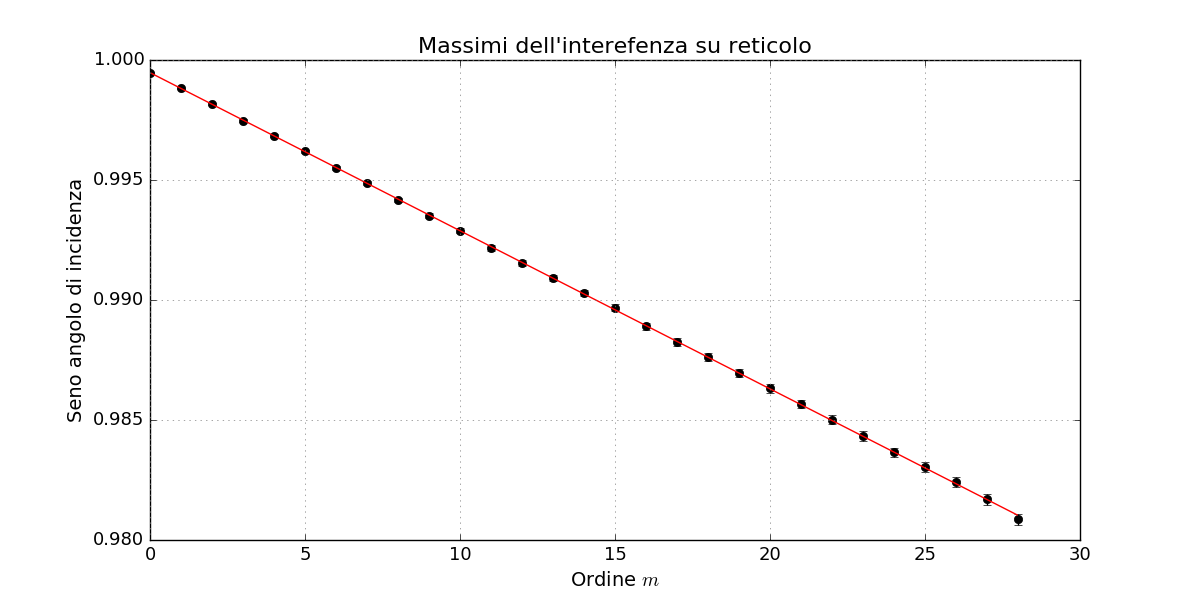
\includegraphics[scale=.5]{plot.png}
\caption{Seno dell'angolo di interferenza in funzione dell'ordine.}
\label{interferenza}
\end{figure}

%Errore troppo grande dovuto a scelta di errore su d
Dal parametro $a$ si ricava il valore di $\lambda = 660 \pm 30 \, nm$ da confrontare con quello teorico del laser $\lambda = 636.3 \, nm$, i due valori non sono compatibili.

\section{Parte B - Misura della lunghezza d'onda della riga verde del mercurio}
\subsection{Calibrazione interferometro}

\begin{figure}[!htb]
  \centering
  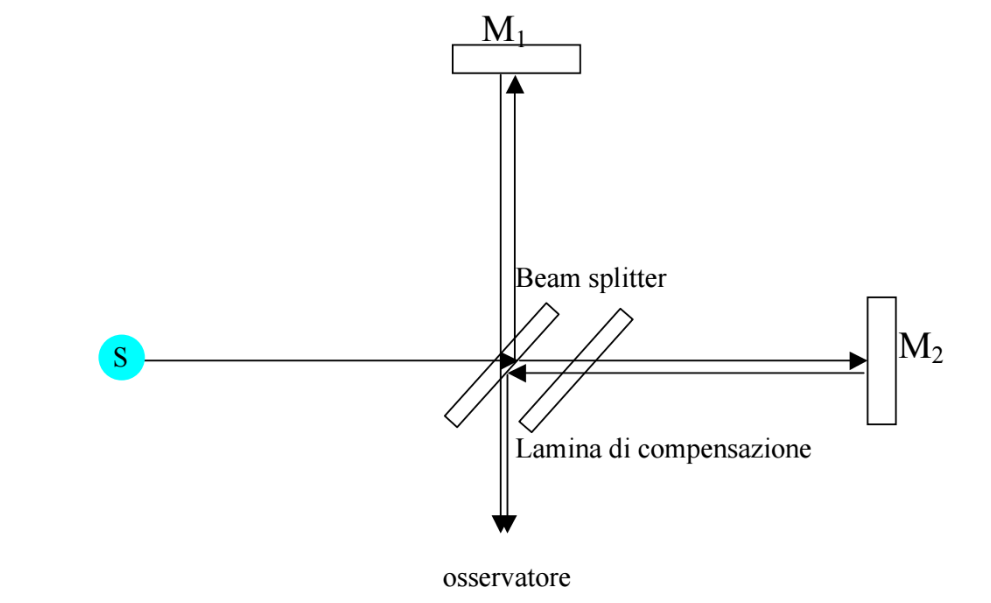
\includegraphics[scale=.5]{interferometro.png}
\caption{Disegno schematico dell'interferometro di Michelson.}
\label{int}
\end{figure}

L'interferometro di Michelson in dotazione è dotato di una vita micrometrica che permette di spostare lo specchio $M1$ (vedi figura \ref{int}), è necessario prima misurare quale sia il rapporto tra il passo della vite e lo spostamento effettivo dello specchio, cioè misurare il fattore di demoltiplica della leva. \\
Per fare ciò si utilizza una sorgente laser He-Ne di lunghezza d'onda nota e si misura lo spostamento della vite necessario perché 30 frange passino per un certo punto dello schermo. Si sono eseguite tre misure riportate nella tabella \ref{calibrazione}, una per ognuno dei componenti del gruppo.\\

Dalla formula $2 \Delta X = m \lambda$ si è ricavato $\Delta X$ e quindi il fattore di demoltiplica $\eta = \frac{\Delta X}{\Delta s}$, dove $\Delta s$ è lo spostamento letto sulla vite micrometrica.

\subsection{Misura di lunghezza d'onda}
Si è cambiata la sorgente luminosa, si è inserita la lampada al mercurio al posto del laser He-Ne, si è aspettato il tempo sufficiente perché ci fosse termalizzazione e si è inserito il filtro verde per selezionare la riga (essere più specifici).\\
Si sono poi eseguite tre misure (una per ogni componente del gruppo) del numero di giri della vita micrometrica necessari perché 50 frange di interferenza passassero per un determinato punto dello schermo. Da queste sempre grazie alla formula precedente si è trovata la lunghezza d'onda cercata.

\section{Conclusioni}

\end{document}